% End-to-end sequence diagram for the Cloud RAN AI Sandbox use case.
% Build:  cd docs/diagrams && pdflatex sequence.tex && pdftoppm -png -r 110 -singlefile sequence.pdf sequence
\documentclass[tikz,border=14pt]{standalone}
\usepackage[scaled]{helvet}
\renewcommand\familydefault{\sfdefault}
\usepackage[T1]{fontenc}
\usetikzlibrary{arrows.meta,positioning,calc}

\definecolor{ink}{HTML}{1F2328}
\definecolor{muted}{HTML}{59636E}
\definecolor{rule}{HTML}{D0D7DE}
\definecolor{head}{HTML}{F6F8FA}
\definecolor{start}{HTML}{DAFBE1}   \definecolor{startline}{HTML}{1A7F37}
\definecolor{fault}{HTML}{FFEBE9}   \definecolor{faultline}{HTML}{CF222E}
\definecolor{rca}{HTML}{DDF4FF}     \definecolor{rcaline}{HTML}{0969DA}
\definecolor{heal}{HTML}{FBEFFF}    \definecolor{healline}{HTML}{8250DF}
\definecolor{note}{HTML}{FFF8C5}    \definecolor{noteline}{HTML}{D4A72C}

\newcommand{\lanegap}{3.25}
\newcommand{\rowh}{0.62}
% lane index -> x
\newcommand{\X}[1]{#1*\lanegap}
% \msg{from}{to}{row}{label}         request (solid)
% \rep{from}{to}{row}{label}         reply (dashed)
\newcommand{\msg}[4]{%
  \draw[-{Stealth[length=2.2mm]}, ink, line width=0.55pt] ({\X{#1}},{-#3*\rowh}) -- ({\X{#2}},{-#3*\rowh})
    node[midway, above=0.5pt, font=\scriptsize, text=ink, fill=white, fill opacity=0.9, text opacity=1, inner sep=1.2pt, align=center] {#4};}
\newcommand{\rep}[4]{%
  \draw[-{Stealth[length=2.2mm,open]}, muted, dashed, line width=0.5pt] ({\X{#1}},{-#3*\rowh}) -- ({\X{#2}},{-#3*\rowh})
    node[midway, above=0.5pt, font=\scriptsize, text=muted, fill=white, fill opacity=0.9, text opacity=1, inner sep=1.2pt, align=center] {#4};}
% \note{lane}{row}{text}
\newcommand{\note}[3]{%
  \node[draw=noteline, fill=note, rounded corners=1.5pt, font=\scriptsize, text=ink, inner sep=2.5pt,
        align=center] at ({\X{#1}},{-#2*\rowh}) {#3};}
% \phase{top row}{bottom row}{fill}{line}{title}
\newcommand{\phase}[5]{%
  \fill[#3] ({-1.55},{-#1*\rowh+0.34}) rectangle ({\X{10}+1.55},{-#2*\rowh-0.36});
  \draw[#4, line width=1.4pt] ({-1.55},{-#1*\rowh+0.34}) -- ({-1.55},{-#2*\rowh-0.36});
  \node[anchor=north west, font=\footnotesize\bfseries, text=#4] at ({-1.45},{-#1*\rowh+0.30}) {#5};}

\begin{document}
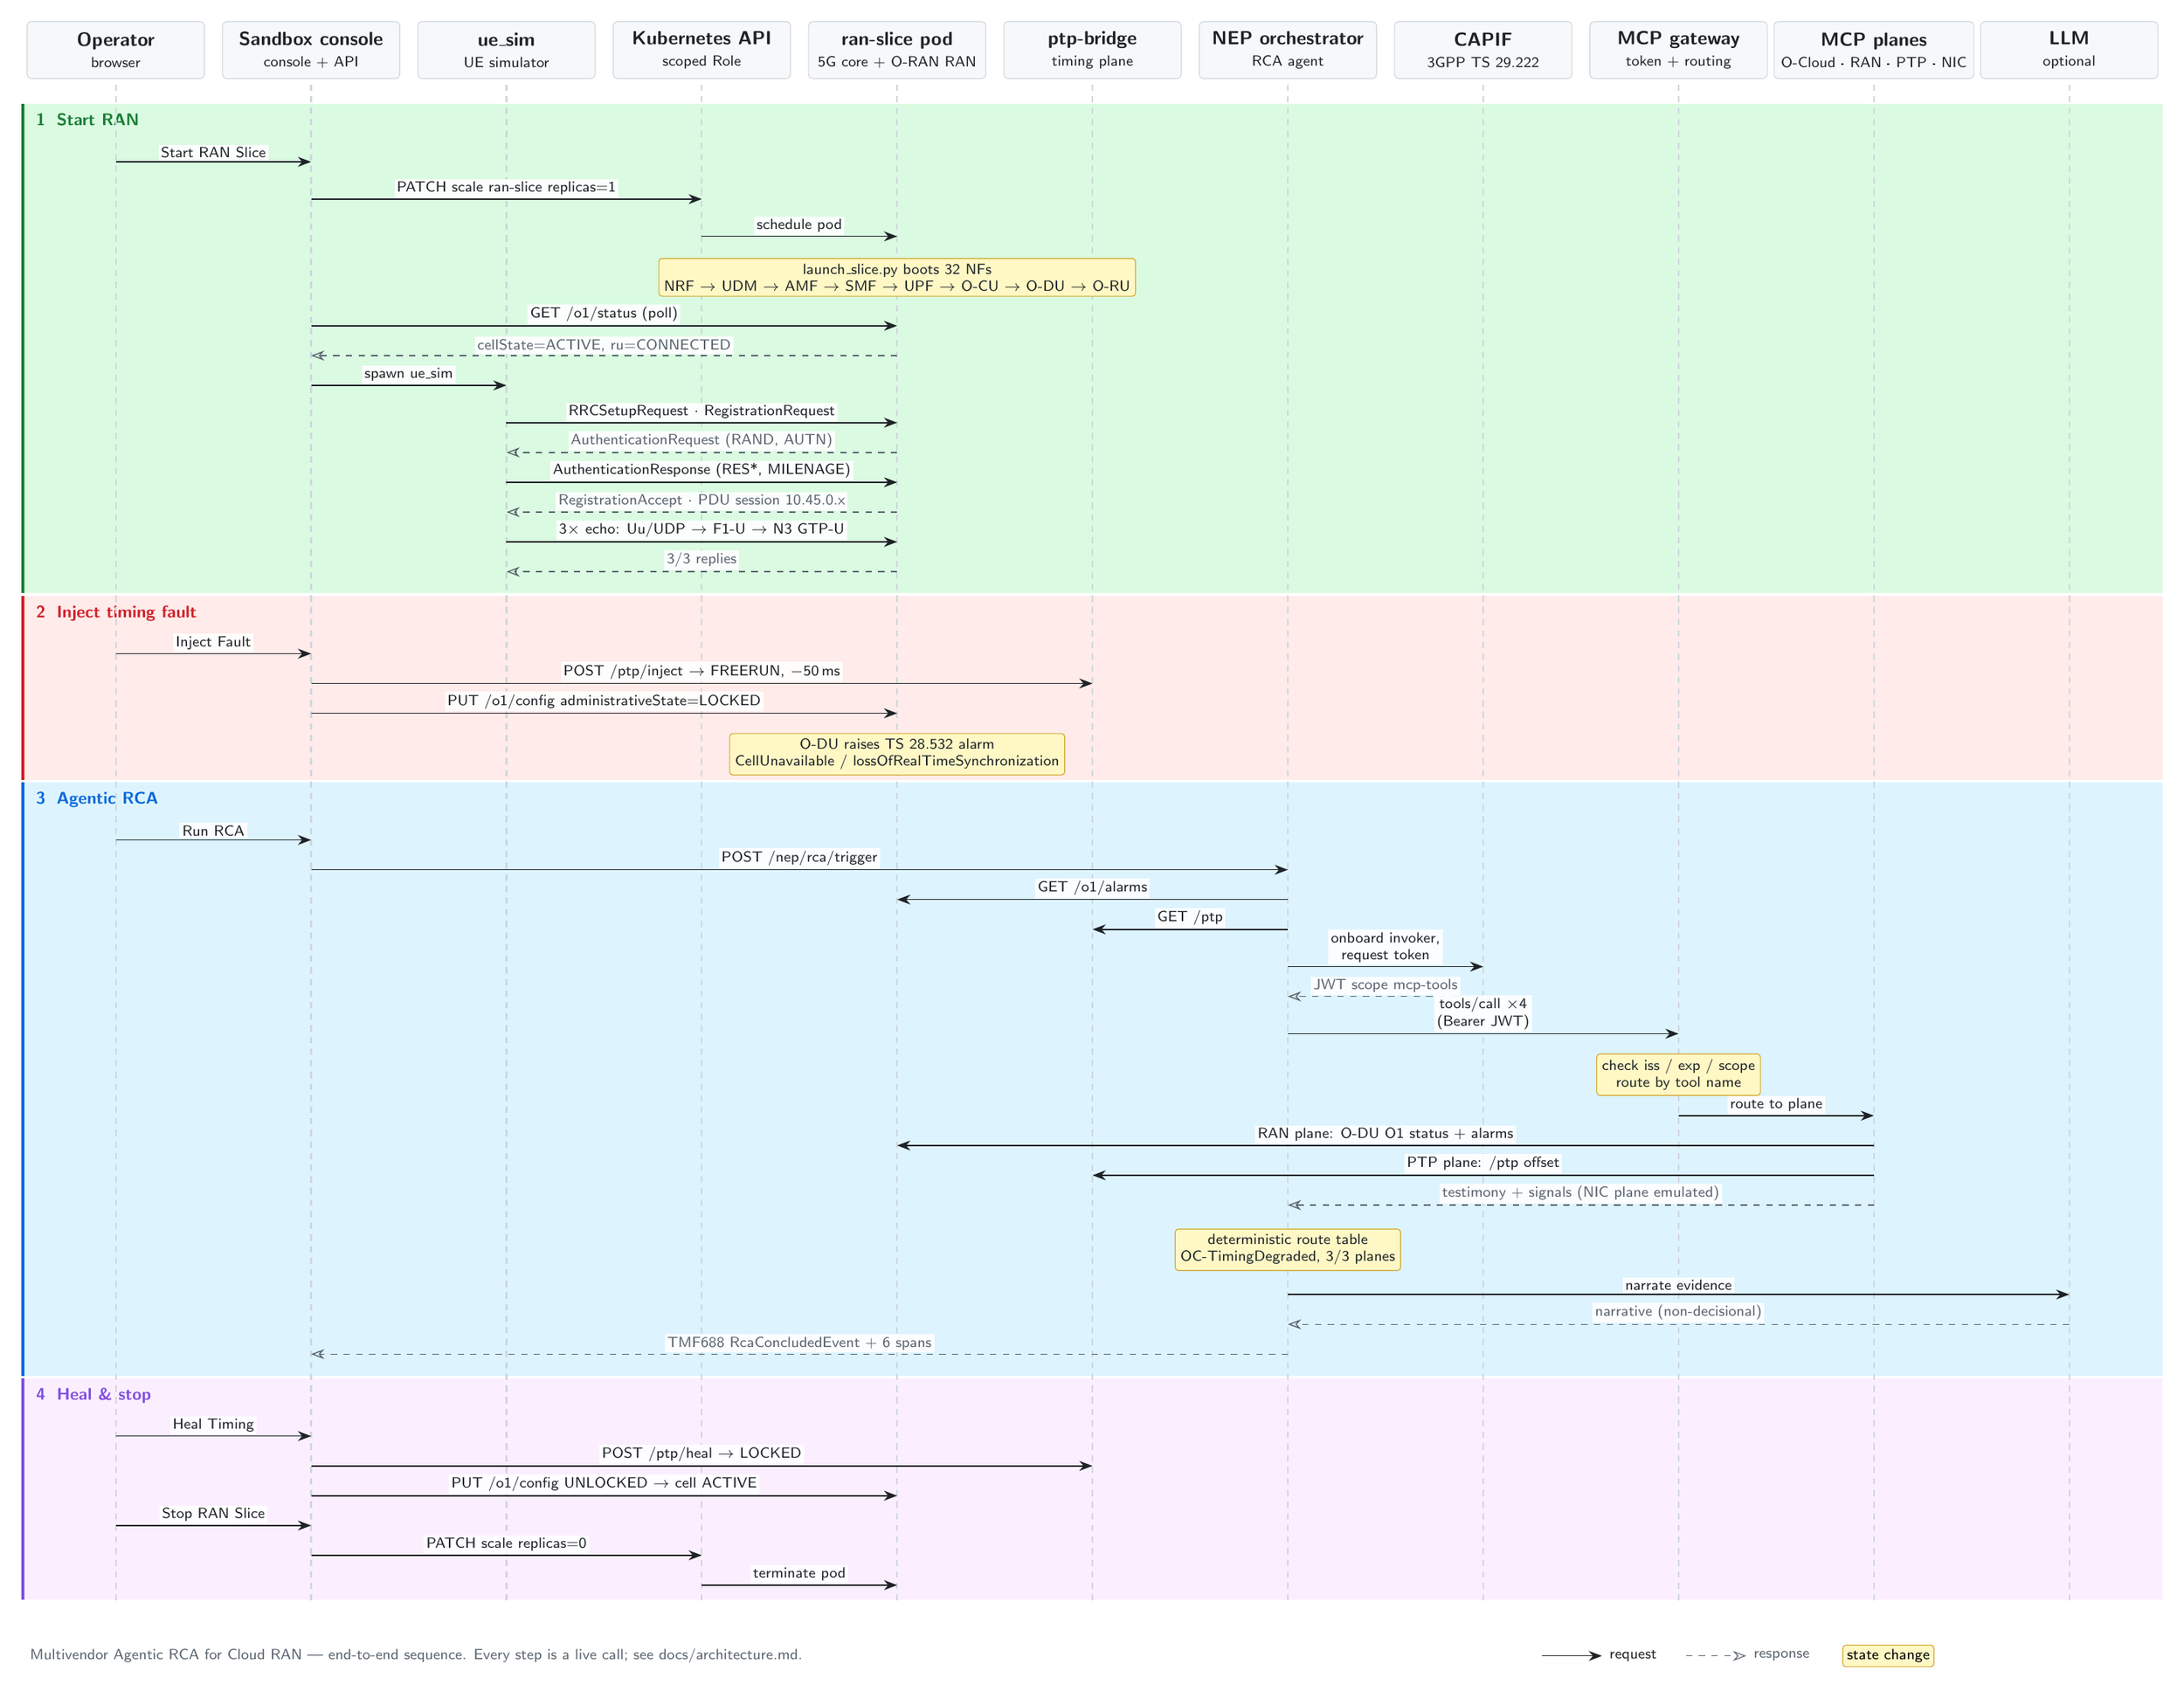
\begin{tikzpicture}[x=1cm,y=1cm]

% ---------- phase bands (drawn first, behind everything)
\phase{1}{13}{start}{startline}{1 \;Start RAN}
\phase{14.2}{18}{fault}{faultline}{2 \;Inject timing fault}
\phase{19.2}{34}{rca}{rcaline}{3 \;Agentic RCA}
\phase{35.2}{40}{heal}{healline}{4 \;Heal \& stop}

% ---------- lifelines
\foreach \i/\name in {0/{Operator\\[-1pt]\scriptsize\mdseries browser},
                      1/{Sandbox console\\[-1pt]\scriptsize\mdseries console + API},
                      2/{ue\_sim\\[-1pt]\scriptsize\mdseries UE simulator},
                      3/{Kubernetes API\\[-1pt]\scriptsize\mdseries scoped Role},
                      4/{ran-slice pod\\[-1pt]\scriptsize\mdseries 5G core + O-RAN RAN},
                      5/{ptp-bridge\\[-1pt]\scriptsize\mdseries timing plane},
                      6/{NEP orchestrator\\[-1pt]\scriptsize\mdseries RCA agent},
                      7/{CAPIF\\[-1pt]\scriptsize\mdseries 3GPP TS 29.222},
                      8/{MCP gateway\\[-1pt]\scriptsize\mdseries token + routing},
                      9/{MCP planes\\[-1pt]\scriptsize\mdseries O-Cloud · RAN · PTP · NIC},
                      10/{LLM\\[-1pt]\scriptsize\mdseries optional}} {
  \draw[rule, line width=0.8pt, dash pattern=on 3pt off 2.5pt] ({\X{\i}},0.05) -- ({\X{\i}},{-40.6*\rowh});
  \node[draw=rule, fill=head, rounded corners=2pt, minimum width=2.95cm, minimum height=0.95cm,
        align=center, font=\small\bfseries, text=ink] at ({\X{\i}},0.62) {\name};
}

% ---------- 1. Start   (lanes: 0 op, 1 sb, 2 ue, 3 k8s, 4 slice, 5 ptp, 6 nep, 7 capif, 8 gw, 9 planes, 10 llm)
\msg{0}{1}{2}{Start RAN Slice}
\msg{1}{3}{3}{PATCH scale ran-slice replicas=1}
\msg{3}{4}{4}{schedule pod}
\note{4}{5.1}{launch\_slice.py boots 32 NFs\\NRF $\to$ UDM $\to$ AMF $\to$ SMF $\to$ UPF $\to$ O-CU $\to$ O-DU $\to$ O-RU}
\msg{1}{4}{6.4}{GET /o1/status (poll)}
\rep{4}{1}{7.2}{cellState=ACTIVE, ru=CONNECTED}
\msg{1}{2}{8}{spawn ue\_sim}
\msg{2}{4}{9}{RRCSetupRequest $\cdot$ RegistrationRequest}
\rep{4}{2}{9.8}{AuthenticationRequest (RAND, AUTN)}
\msg{2}{4}{10.6}{AuthenticationResponse (RES*, MILENAGE)}
\rep{4}{2}{11.4}{RegistrationAccept $\cdot$ PDU session 10.45.0.x}
\msg{2}{4}{12.2}{3$\times$ echo: Uu/UDP $\to$ F1-U $\to$ N3 GTP-U}
\rep{4}{2}{13}{3/3 replies}

% ---------- 2. Fault
\msg{0}{1}{15.2}{Inject Fault}
\msg{1}{5}{16}{POST /ptp/inject $\to$ FREERUN, $-$50\,ms}
\msg{1}{4}{16.8}{PUT /o1/config administrativeState=LOCKED}
\note{4}{17.9}{O-DU raises TS 28.532 alarm\\CellUnavailable / lossOfRealTimeSynchronization}

% ---------- 3. RCA
\msg{0}{1}{20.2}{Run RCA}
\msg{1}{6}{21}{POST /nep/rca/trigger}
\msg{6}{4}{21.8}{GET /o1/alarms}
\msg{6}{5}{22.6}{GET /ptp}
\msg{6}{7}{23.6}{onboard invoker,\\request token}
\rep{7}{6}{24.4}{JWT scope mcp-tools}
\msg{6}{8}{25.4}{tools/call $\times$4\\(Bearer JWT)}
\note{8}{26.5}{check iss / exp / scope\\route by tool name}
\msg{8}{9}{27.6}{route to plane}
\msg{9}{4}{28.4}{RAN plane: O-DU O1 status + alarms}
\msg{9}{5}{29.2}{PTP plane: /ptp offset}
\rep{9}{6}{30}{testimony + signals (NIC plane emulated)}
\note{6}{31.2}{deterministic route table\\OC-TimingDegraded, 3/3 planes}
\msg{6}{10}{32.4}{narrate evidence}
\rep{10}{6}{33.2}{narrative (non-decisional)}
\rep{6}{1}{34}{TMF688 RcaConcludedEvent + 6 spans}

% ---------- 4. Heal & stop
\msg{0}{1}{36.2}{Heal Timing}
\msg{1}{5}{37}{POST /ptp/heal $\to$ LOCKED}
\msg{1}{4}{37.8}{PUT /o1/config UNLOCKED $\to$ cell ACTIVE}
\msg{0}{1}{38.6}{Stop RAN Slice}
\msg{1}{3}{39.4}{PATCH scale replicas=0}
\msg{3}{4}{40.2}{terminate pod}

% ---------- legend
\begin{scope}[shift={({\X{7.3}},{-42.1*\rowh})}]
  \draw[-{Stealth[length=2.2mm]}, ink, line width=0.55pt] (0,0) -- (1,0) node[right, font=\scriptsize, text=ink] {request};
  \draw[-{Stealth[length=2.2mm,open]}, muted, dashed] (2.4,0) -- (3.4,0) node[right, font=\scriptsize, text=muted] {response};
  \node[draw=noteline, fill=note, rounded corners=1.5pt, font=\scriptsize, inner sep=2pt, right] at (5,0) {state change};
\end{scope}
\node[anchor=west, font=\scriptsize, text=muted] at (-1.55,{-42.1*\rowh})
  {Multivendor Agentic RCA for Cloud RAN — end-to-end sequence. Every step is a live call; see docs/architecture.md.};

\end{tikzpicture}
\end{document}
